\documentclass{article}
\usepackage{tikz}
\usepackage{amsmath}
\graphicspath{ {images/} }
\begin{document}

\section{Transformación del campo lejano a partir del campo cercano medido en coordenadas esféricas}

Pese a haber explicado la obtención del campo lejano a partir de medidas realizadas sobre un plano en coordenadas cartesianas. Nuestro verdadero interés está en poder obtener el campo lejano a partir de medidas del campo cercano en coordenadas esféricas.
Ya que, de forma típica, los diagramas de radiación de campo lejano suelen representarse sobre el sistema de coordenadas esférico. \\

Estando ambos sistemas de coordenadas relacionados de la siguiente forma:


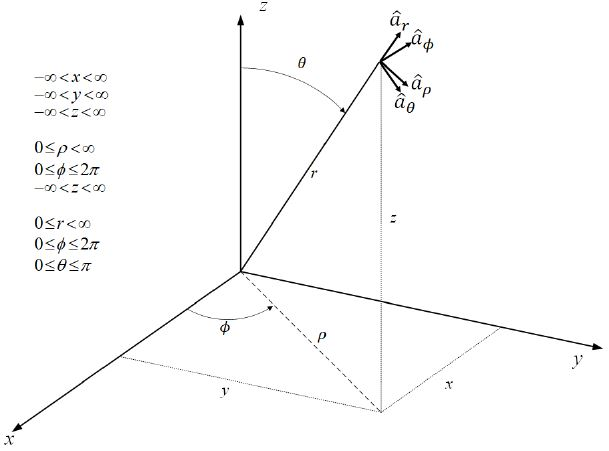
\includegraphics[scale=0.65]{relacion_esfericas_cartesianas}

\\ 

Aunque trabajar con coordenadas esféricas es más complicado, la razón principal para utilizarlas radica en que el sistema de medición de las antenas bajo prueba emplea este tipo de coordenadas.\\
Esto se debe a  que el propósito de la medición es caracterizar el comportamiento de la antena bajo estudio en todas las direcciones. Para lo cual,  la mejor forma es emplear un sistema de coordenadas esférico que tenga como origen la propia antena sobre la que deseamos obtener medidas.
\\

Una vez introducido y justificado el uso de coordenadas esféricas, es necesario enfocarnos en plantear nuestro problema de manera que podamos resolverlo utilizando este sistema de coordenadas. \\
Para ello, lo primero que debemos tener en cuenta, es que vamos a tratar con ecuaciones de ondas esféricas. Por lo que es necesario disponer de, almenos, la base fundamental de estas ecuaciones.

\section{Teoria básica de ecuaciones esféricas}

Dado que nuestro problema pertenece a un sistema de coordenadas curvilíneo,  el uso de ecuaciones diferenciales sobre nuestro campo presenta dificultades añadidas. \\
Sin embargo, podemos reducir su complejidad aprovechando una característica de estas ecuaciones. La cual nos permite tratar la resolución de ecuaciónes diferenciales hechas sobre un vector (en nuestro caso, el campo eléctrico), si consideramos que podemos obtener dicho vector a partir dos vectores parciales.\\
No obstante, esta propiedad  solo puede aplicarse en caso de que los vectores parciales sean derivables a partir de una función puramente escalar que satisfaga las ecuaciones de onda vectoriales. \\

Adelantándonos un poco a lo explicado a continuación. Nosotros  siempre vamos a tratar con vectores que pueden descomponerse en vectores parciales. Cosa que vamos a demostrar en el siguiente punto.No obstante, por el momento, nos basta con saber que ciertos vectores pueden ser descompuestos en otros parciales; y que este caso particular es el que nos interesa estudiar.
\\
Dicho todo esto, la condición fundamental que permite que hagamos uso de estos vectores parciales, es que cumplan las ecuaciones de onda vectoriales. Motivo por el cual vamos a centrar nuestra atención sobre estas ecuaciones.

\subsection{ecuaciones de onda vectoriales}

Estas ecuaciones son, por si solas, un objeto de estudio bastante complejo.  No obstante, a nosotros solo nos interesa su uso aplicado a nuestro caso particular.
Lo cual nos va a permitir hacer una serie de simplificaciones que iremos detallando y justificando sobre la marcha.\\

De entrada, vamos a partir rescatando la idea de que vamos a hacer uso  de una cámara anecoica para relizar las medidas. Lo que significa que vamos a tener un entorno de medición con unas condiciones prácticamente iguales a las del vacío. \\
Por tanto, disponemos de un dominio cerrado (es decir,  un conjunto que incluye todos sus puntos, incluidos los puntos límite; y cuyo complemento es un conjunto abierto) con un medio de propagación isotrópico sin fuentes.\\

Este entorno en particular resulta ser el más favorable a la hora de tratar con ecuaciones de onda vectoriales. Ya que cualquiera de los vectores de campo ($E$,$B$,$D$ y $H$),  el vector potencial $A$ o  los vectores de potencia de Hertz, satisfacen una única ecuación diferencial. La cual cumplen todos ellos; y que toma la siguiente forma:
\begin{equation}
\nabla^2C - \mu\varepsilon\frac{\partial^2C}{\partial^2{t}} - \mu\sigma\frac{\partial C}{\partial{t}} = 0\
\label{eq-esfvec-general}
\end{equation}
Donde $C$ representa cualquiera de los posibles vectores citados anteriormente.\newpage
A partir de esta ecuación general, lo primero que podemos hacer es emplear la propiedad de que las ecuaciones de onda esférica son lineales. Esto nos permite simplificar la implicación del tiempo de nuestra ecuación.\\
Ya que, gracias a la linealidad, podemos reconstruir aquellos vectores que tengan una variación arbitraria con el tiempo a partir de soluciones armónicas. Permitiendonos reescribir la ecuación sin perder con ello la generalización en nuestra expresión. \\

Es decir, podemos afirmar que nuestro vector  $C$ únicamente varía con respecto al tiempo en base al factor $e^{-jwt}$. 
Además, podemos simplificar más nuestra expresión si recordamos que el operador laplaciano ($\nabla^2$) aplicado sobre un vector cualquiera equivale a lo siguiente:
\begin{equation}
\nabla^2C =\nabla\nabla C - \nabla\times\nabla\times C + k^2C
\label{eq-nabla-sobre-vector}
\end{equation}
Con $k^2$ = $\mu\varepsilon w^2 + j\mu\sigma w$ .\\

Por lo que, aplicando todo esto, podemos reescribir  \eqref{eq-nabla-sobre-vector} de la siguiente forma:
\begin{equation}
\nabla\nabla C - \nabla \times \nabla \times C + k^2 C = 0\label{eq-esfvec-simplificada}
\end{equation}
Para poder tratar con esta ecuacíón, disponemos de dos alternativa: 

\begin{enumerate}
    \item Podemos optar por el camino tradicional. El cual pasa por resolver \eqref{eq-esfvec-simplificada} como un sistema de tres ecuaciones escalares.
    \item Podemos simplificar la resolución de \eqref{eq-esfvec-simplificada} resolviendo tan solo tres ecuaciones escalares independientes. Pero solo podemos considerar esta opción \textbf{si y solo si} podemos obtener $C$ a partir de sus componentes rectangulares.
\end{enumerate}

De estos dos métodos, siempre vamos a preferir el segundo. Ya que la resolución del sistema implica una alta complejidad en los cálculos. Sobretodo si la comparamos con la resolución de las tres ecuaciones independientes. \\

Volviendo a centrar la atención a nuestro problema en particular, tenemos la opción de aplicar el segundo método. Ya que siempre vamos a ser capaces de obtener el campo medido a partir de sus componentes rectangulares.\\
Lo cual se justifica dado que nuestras medidas van a cumplir siempre las propiedades de ortogonalidad.\\

Por lo que, llegados a este punto, podemos reescribir \eqref{eq-esfvec-simplificada} de la siguiente manera:
\begin{equation}
\nabla^2C_{j} + k^2C_{j} = 0
\label{eq-nabla-cuadrado-coordenada}
\end{equation}
Donde $C_{j}$ hace referencia las componentes ($x$,$y$,$z$) del vector $C$.\\
\newpage
A partir de este resultado, tendremos tantas soluciones como vectores $C$ existan. Por lo que, de ahora en adelante, vamos a considerar $\psi$ como una función escalar que es solución de \eqref{eq-nabla-cuadrado-coordenada}.\\
\begin{equation}
\nabla^2\psi + k^2\psi = 0
\label{eq-nabla-cuadrado-coordenada-con-una-soculicon-por-vector-C}
\end{equation}

De esta forma; y considerando  '$a$' como un vector unitario constante cualquiera, podemos escribir tres vectores independientes a partir de $\psi$. Los cuales son, de hecho, solución de \eqref{eq-esfvec-simplificada}:
\begin{subequations}
\begin{align}
    L&= \nabla\psi \label{eq:Lirrotacional}\\
    M&= \nabla\times a\psi\\
    N&=\frac{1}{k}\nabla\times N
\end{align}
\end{subequations}

Una vez planteadas estas tres ecuaciones, vamos a detenernos brevemente para citar algunas propiedades presentes en ellos.\\
De entrada, gracias a que '$a$' es un vector unitario, podemos reescribir $M$ de la siguiente manera:    
\begin{equation}
M= L \times a = \frac{1}{k}\nabla \times N
\label{eq-M-reescrito}
\end{equation}
Además,  para nuestra posible solución $\psi$, el vector $M$ es perpendicular a $L$. O lo que es lo mísmo, $L\cdot M=0$.\\

Al margen de a estas propiedades de $M$, por definición, las ecuaciones $L$, $M$ y $N$ presentan algunas características muy interesantes.\\
Por un lado, para $L$ se cumplen las siguientes dos propiedades:
\begin{align}
    \nabla  \times L &=0 \\
    \nabla  \cdot L  &=\nabla^2\psi = -k^2 \psi
\end{align}
Donde hemos aplicado la ecuación \eqref{eq:Lirrotacional} para obtener el caracter irrotacional del vector $\vec{L}$ y convertir su divergencia en un laplaciano. \\
Con respecto a  $M$ y $N$, si rescatamos la idea de que estamos tratando vectores de campo eléctrico, significa que tanto $M$ como $N$ son capaces de crear un campo magnético.\\
Como además estamos considerando vectores pertenencientes a un medio prácticamente igual al vacío, significa que sus divergencias son nulas para cualquier punto dentro de este dominio.\\
O lo que es lo mísmo,  los vectores $M$ y $N$ cumplen la condición de campo solenoidal:
\begin{align}
    \nabla\cdot M &= 0
    \label{M-cumplen-ser-campo-solenoidal}\\
    \nabla\cdot N &= 0
    \label{N-cumplen-ser-campo-solenoidal}
\end{align}
\newpage
Una vez estudiadas todas estas propiedades de los vectores $L$, $M$ y $N$. Debemos tener en cuenta que existen 3 tipos de soluciones para una ecuación diferencial, la general, la particular y la singular.\\
En nuestro caso, dado que estamos suponiendo que para cada punto existe una única solución $C$, lo que hemos estado manejando hasta ahora son, por definición, las soluciones particulares de \eqref{eq-nabla-cuadrado-coordenada-con-una-soculicon-por-vector-C}. \\
Asique, de ahora en adelante, vamos a hacer uso de la notación $\psi_{n}$ para hacer referencia a cualquiera de estas soluciones particulares de la ecuación diferencial. Existiendo entonces para cada solución  $\psi_{n}$; un conjunto de vectores $L_{n}$, $M_{n}$ y $N_{n}$.
\\

Llegados a este punto, ya tenemos todos los resultados que nos interesaban de las ecuaciones de onda vectoriales. De todo lo visto, realmente solo nos interesan los valores de   $M_{n}$ y $N_{n}$.\\
Esto se debe a que en caso de que la función dada sea solenoidal (su divergencia es nula en el dominio), su extensión se puede obtener únicamente en términos de  $M_{n}$ y $N_{n}$. 
\\

Recapitulando entonces con la idea de poder simplficar las ecuaciones de onda esférica. Hemos encontrado los vectores parciales que nos permiten representar el campo. Es decir, podemos utilizar $M$ y $N$ como vectores parciales de $E$ y $H$.\\

En resumen, si se cumple:
\begin{enumerate}
    \item Que la variación arbitraria del tiempo entra en juego únicamente como un factor armónico $e^{-jwt}$.
    \item Que estamos trabajamos con un medio donde la densidad de cargas libres es nulo en todas partes.
    \item   Que nuestro medio es isotropico.
    \item Podemos caracterizar la conductividad de nuestro medio de forma única con valor $\sigma$.

\end{enumerate}
Solo entonces podremos definir los campos $E$ y $H$ de esta forma:
\begin{equation}
E = \frac{jw\mu}{k^2}\nabla \times H\xrightarrow{}   H= \frac{1}{jw\mu}\nabla \times E
\label{campo-EyH-cumpliendo-simplificacion-con-MnyNn}
\end{equation}
Por lo que, suponiendo que el vector potecial también puede ser representado por una expansión de funciones vectoriales caracteristicas. Entonces podemos escribir el valor del vector potencial como:
\begin{equation}
A = \frac{1}{w}\sum_{n}(a_{n}M_{n}+b_{n}N_{n}+c_{n}L_{n})
\label{vector-potencial-cumpliendo-simplificacion-con-MnyNn}
\end{equation}
Donde los coeficientes $a_{n}, b_{n}, c_{n}$ pueden ser obtenidos a partir de la distribución de carga del campo.

Aqui es donde entran en juego las propiedades de $L_{n}$, $M_{n}$ y $N_{n}$. Ya que gracias  a las propiedades vistas en \eqref{M-cumplen-ser-campo-solenoidal} y \eqref{N-cumplen-ser-campo-solenoidal}; a poder ignorar el vector $L_{n}$; y haciendo uso de la relación $\mu H = \nabla \times A$. Podemos escribir las ecuaciones de campo como:
\begin{align}
    E &= - \sum_{n}(a_{n}M_{n}+b_{n}N_{n})\\
    H &= - \frac{k}{jw\mu}\sum_{n}(a_{n}M_{n}+b_{n}N_{n})
\end{align}
Es decir, ya somos capaces de expresar nuestro campo eléctrico a partir de las funciones de onda esférica $}M_{n}$ y$N_{n}$ y los coeficientes de onda $a_{n}$ y $b_{n}$. \\
Por lo que, podemos definir un campo eléctrico medido en coordenadas esféricas de la siguiente manera:
\begin{equation}
\vec{E}(r,\theta,\phi)=\sum_{n=-Nm}^{Nm}(a_{n}M_{n}(r,\theta,\phi)+b_{n}N_{n}(r,\theta,\phi))
\label{eq-campoE-coordenadas-esfericas}
\end{equation}
\newpage
\section{Método para la obtención del campo lejano}
Hasta ahora hemos hecho referencia a campos. Pero lo que realmente va a interesarnos a partir de ahora es el estudio de los  modos del campo eléctrico.\\
Es por esto que debemos mencionar el desuso  del subíndice  $n$ que hemos venido usando hasta ahora para representar que tratábamos con soluciones particulares de la ecuación diferencial.\\
Ya que a partir de ahora, vamos a referirnos siempre a modos, por lo que usaremos el sumbíndice $m$ y $n$ para ello.\\

Es por esto por lo que de ahora en adelande, en lugar de usar la ecuación del campo eléctrico definida en \eqref{eq-campoE-coordenadas-esfericas}, vamos a reescribirla para poder obtener $\vec{E}(r,\theta,\phi)$ a partir del desarrollo de sus modos:
\begin{equation}
\vec{E}(r,\theta,\phi)=\sum_{m=-M}^{M}\sum_{n=-N}^{N}\big[a_{n}M_{mn}(r,\theta,\phi)+b_{n}N_{mn}(r,\theta,\phi)\big]
\label{eq-campoE-coordenadas-esfericas-a-partir-de-sus-modos}
\end{equation}

TO-DO

\newpage


\end{document}

